% Benchmark overview, 17.4 x 6.8 cm. All photographs are unchanged source assets.
\begingroup%
\definecolor{raBlue}{RGB}{40,86,124}%
\definecolor{raTeal}{RGB}{51,106,99}%
\definecolor{raOrange}{RGB}{150,89,35}%
\begin{tikzpicture}[x=1cm,y=1cm,>=Latex,font=\small,
 photo/.style={inner sep=0pt,outer sep=0pt},
 rule/.style={draw=black!25,line width=.45pt},
 arr/.style={->,line width=.65pt,draw=black!60},
 note/.style={font=\footnotesize,align=center},
 tinylabel/.style={font=\scriptsize,align=center,text=black!70}]
\path[use as bounding box] (0,0) rectangle (17.4,6.8);
% Section headings and restrained separators.
\node[anchor=west,font=\small\bfseries] at (0,6.57) {(a) Start from real photographs};
\node[anchor=west,font=\small\bfseries] at (5.08,6.57) {(b) Four versions of one family};
\node[anchor=west,font=\small\bfseries] at (12.03,6.57) {(c) Search and decide};
\draw[rule] (4.88,.12) -- (4.88,6.75);
\draw[rule] (11.75,.12) -- (11.75,6.75);
% (a) Real image pools and concrete questions.
\node[anchor=west,font=\footnotesize\bfseries,text=raBlue] at (.08,6.02) {Condition \textnormal{--- MVTec AD}};
\node[photo] at (1.25,4.88) {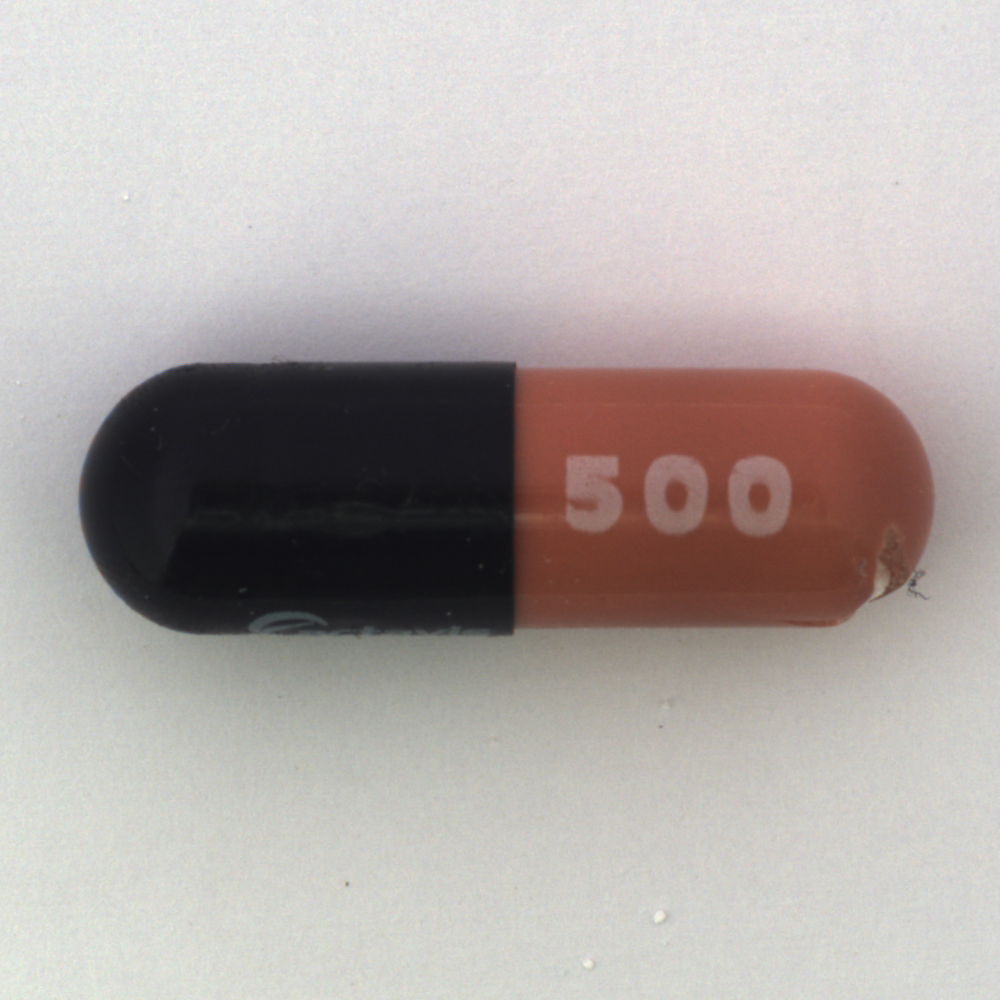
\includegraphics[width=1.9cm]{figures/capsule-original.png}};
\node[photo] at (3.55,4.88) {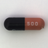
\includegraphics[width=1.35cm]{figures/capsule-preview.png}};
\node[note] at (1.25,3.75) {Original};
\node[note] at (3.55,3.75) {Preview};
\node[anchor=west,font=\footnotesize] at (.08,3.32) {Does the capsule have a crack?};
\node[anchor=west,font=\footnotesize\bfseries,text=raBlue] at (.08,2.85) {Identity \textnormal{--- CO3D}};
\node[photo] at (1.25,1.95) {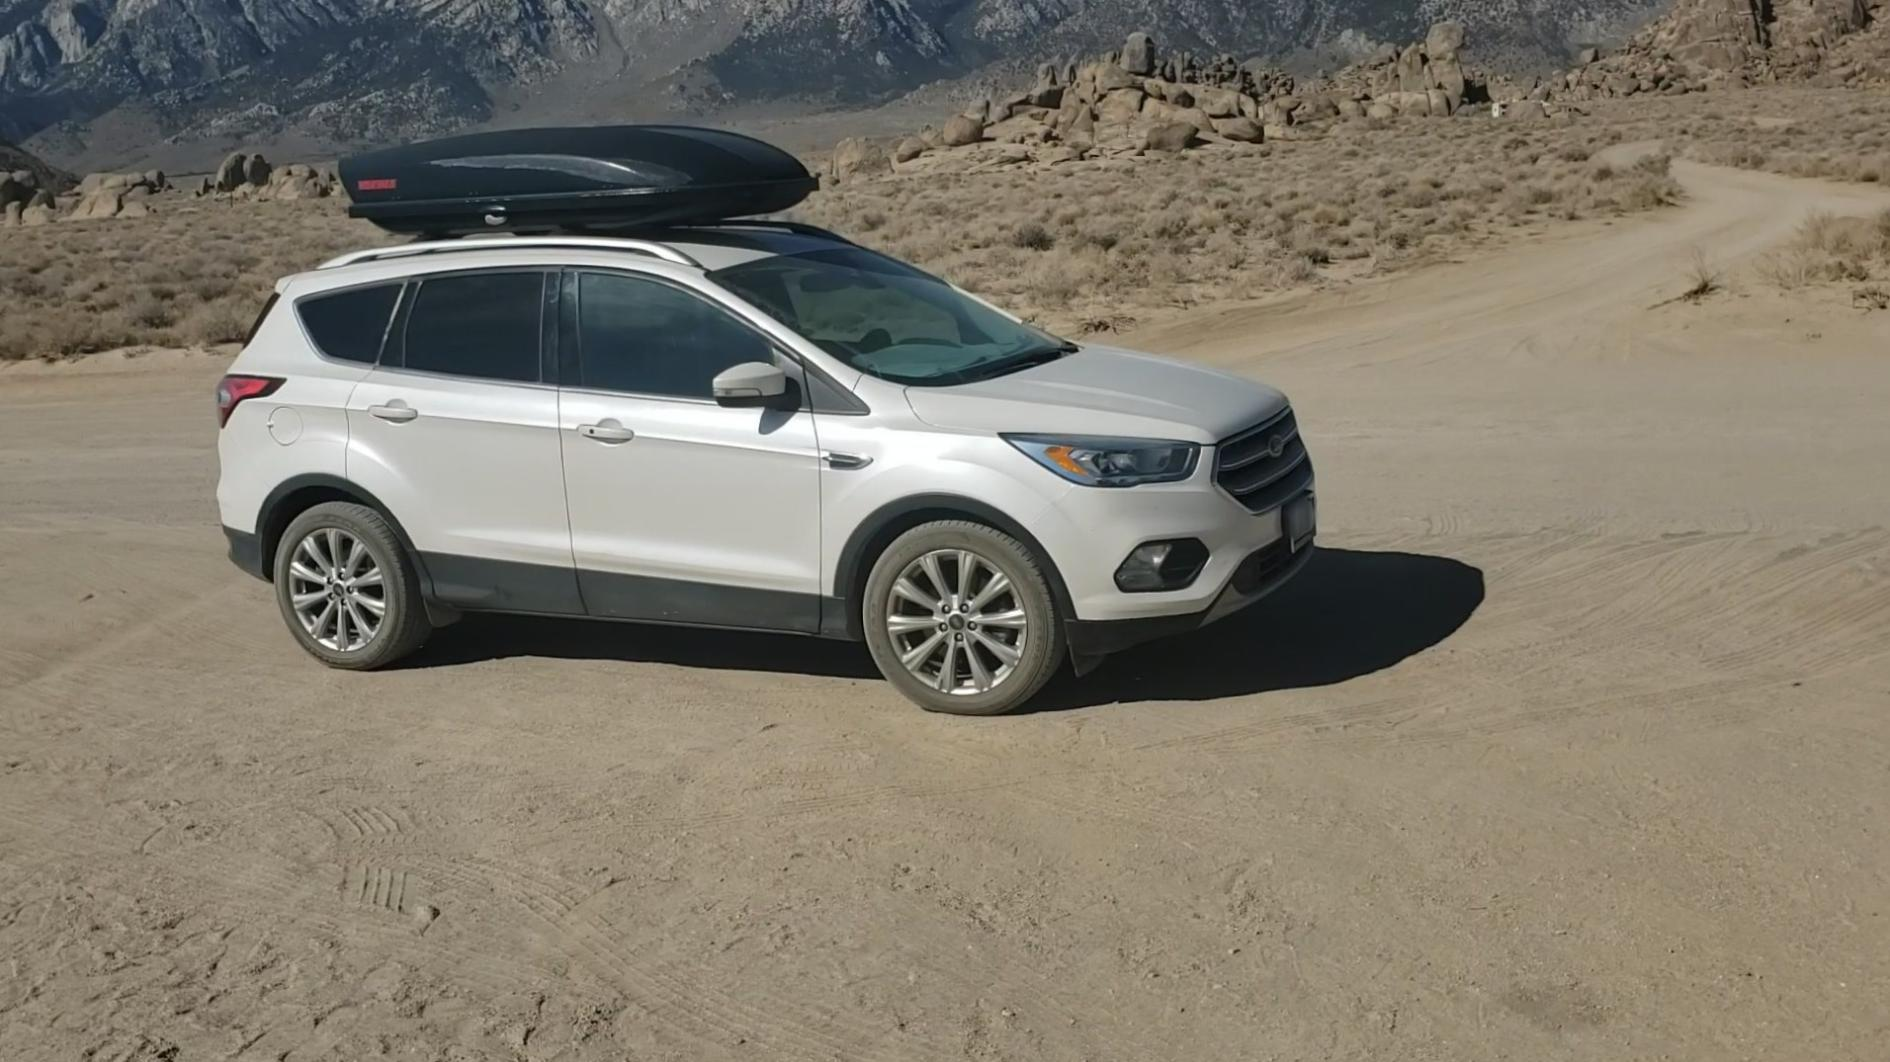
\includegraphics[width=2.15cm]{figures/case-vehicle-a.jpg}};
\node[photo] at (3.55,1.95) {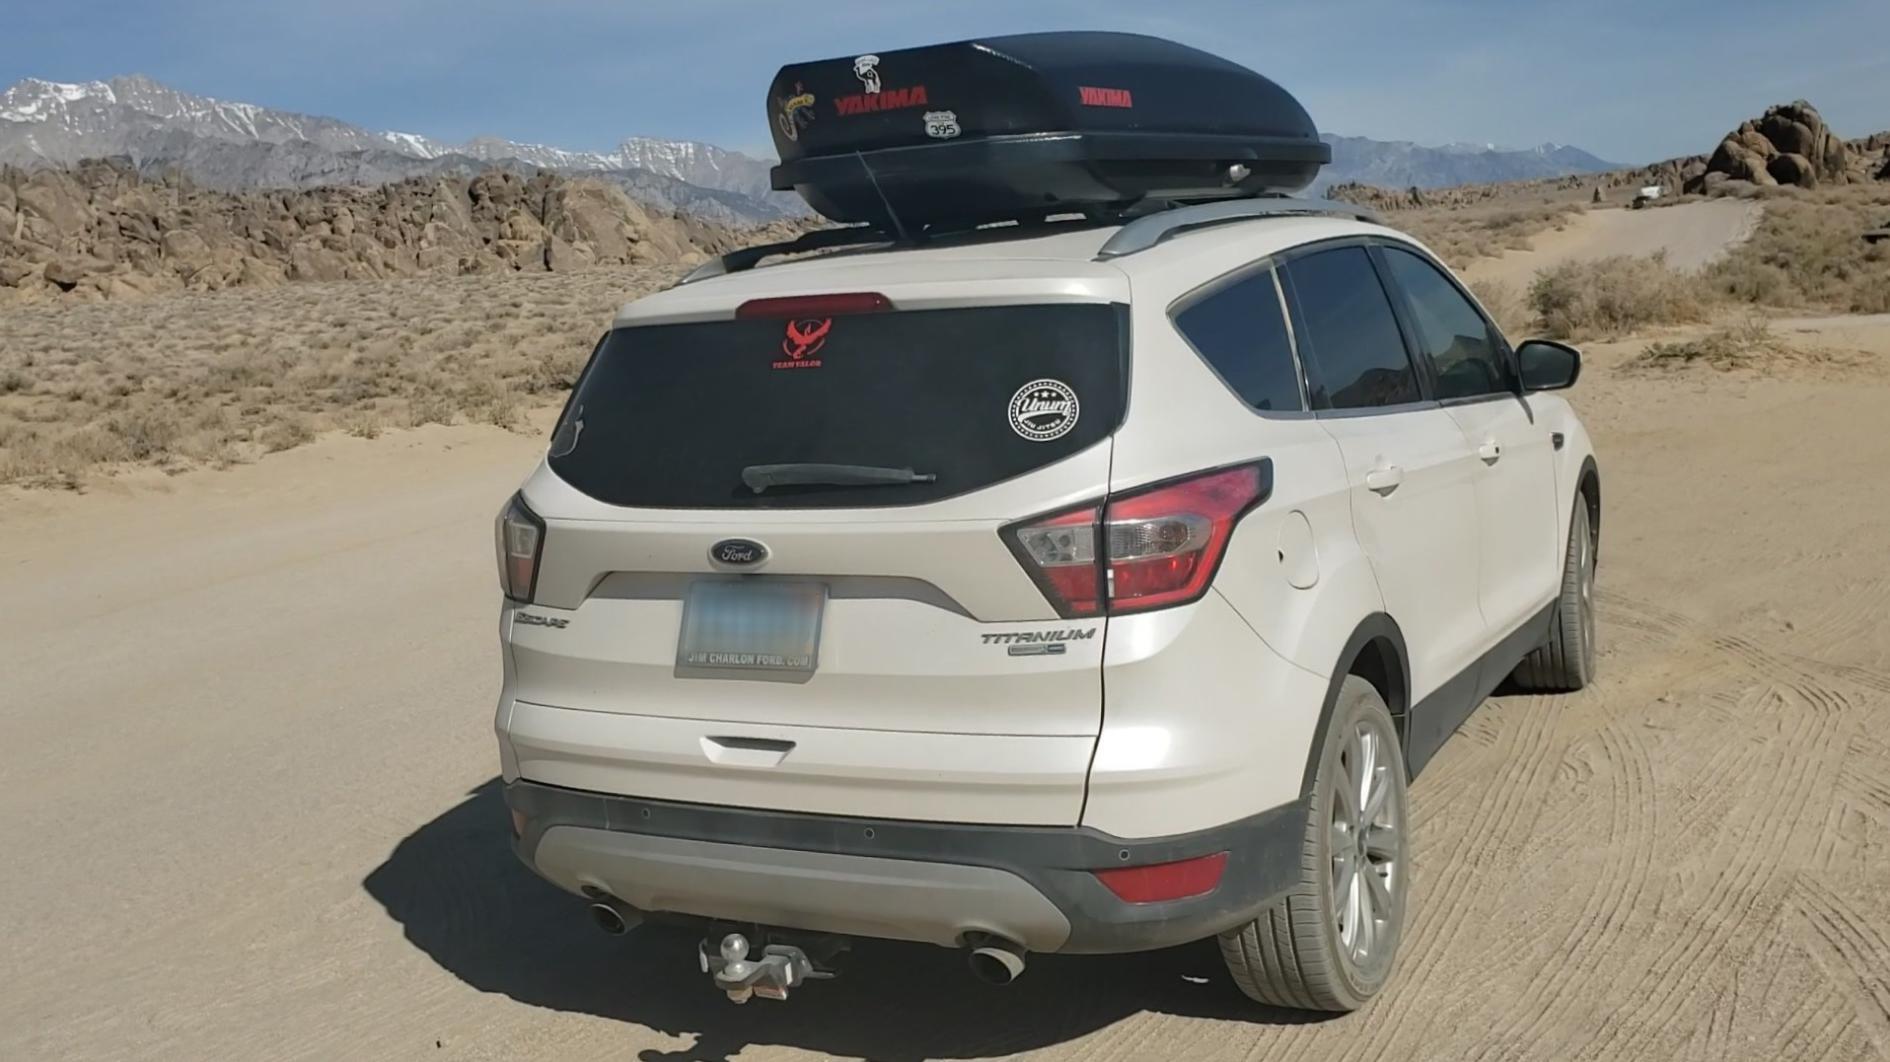
\includegraphics[width=2.15cm]{figures/case-vehicle-b.jpg}};
\node[note] at (1.25,1.16) {Image A};
\node[note] at (3.55,1.16) {Image B};
\node[anchor=west,font=\footnotesize] at (.08,.65) {Do A and B show the same item?};
% (b) Physical state and question fixed; access alone is changed.
\node[anchor=west,font=\footnotesize] at (5.1,6.02) {Same capsule, same claim; different photo access.};
\node[font=\footnotesize\bfseries] at (8.3,5.56) {Initial image};
\node[font=\footnotesize\bfseries] at (10.4,5.56) {Request: original};
\foreach \y in {4.28,3.08,1.88,.68}{\draw[rule] (5.08,\y) -- (11.48,\y);}
% Sufficient.
\draw[draw=raTeal,line width=2.2pt] (5.1,4.46) -- (5.1,5.24);
\node[anchor=west,font=\small\bfseries,text=raTeal] at (5.25,4.99) {Sufficient};
\node[anchor=west,font=\footnotesize] at (5.25,4.61) {Original supplied};
\node[photo] at (8.3,4.85) {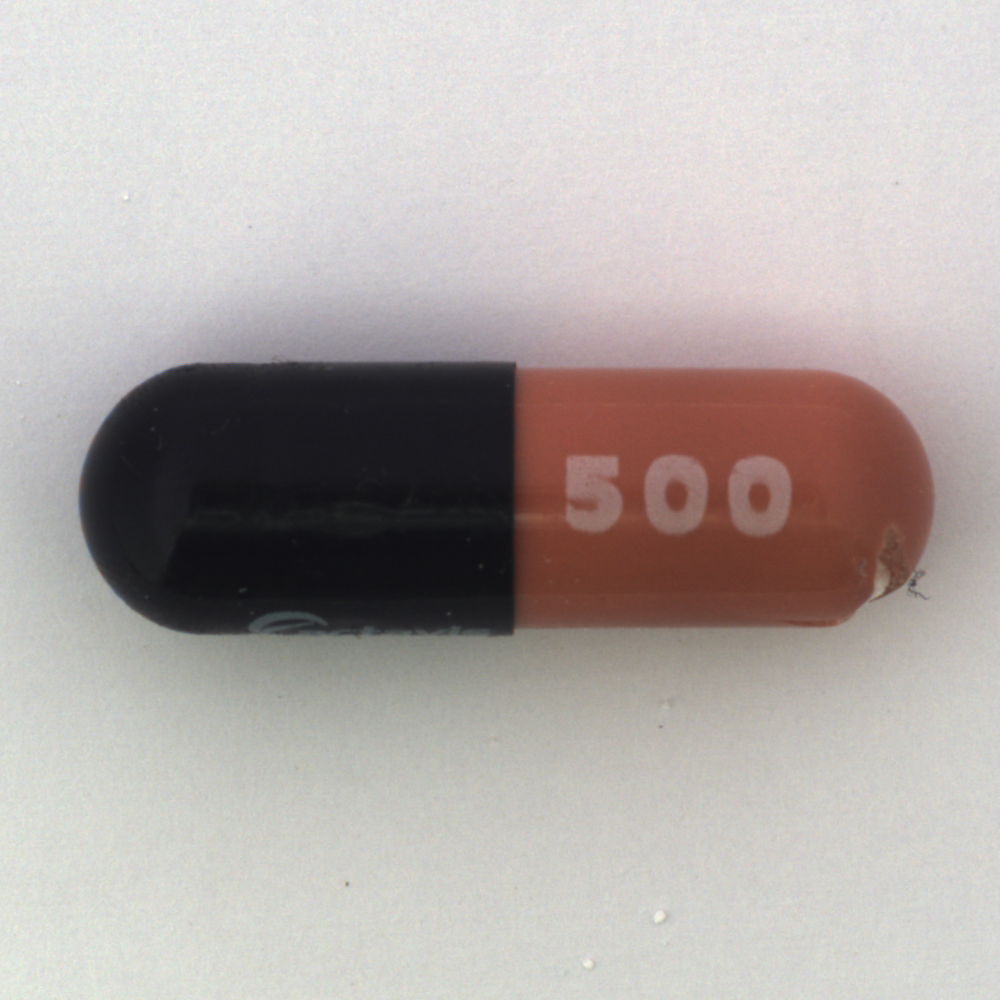
\includegraphics[width=.85cm]{figures/capsule-original.png}};
\node[font=\footnotesize,text=black!60] at (10.4,4.85) {not needed};
% Obtainable.
\draw[draw=raBlue,line width=2.2pt] (5.1,3.26) -- (5.1,4.04);
\node[anchor=west,font=\small\bfseries,text=raBlue] at (5.25,3.79) {Obtainable};
\node[anchor=west,font=\footnotesize] at (5.25,3.41) {Original on request};
\node[photo] at (8.3,3.65) {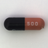
\includegraphics[width=.85cm]{figures/capsule-preview.png}};
\draw[arr,draw=raBlue] (8.88,3.65) -- (9.67,3.65);
\node[photo] at (10.4,3.76) {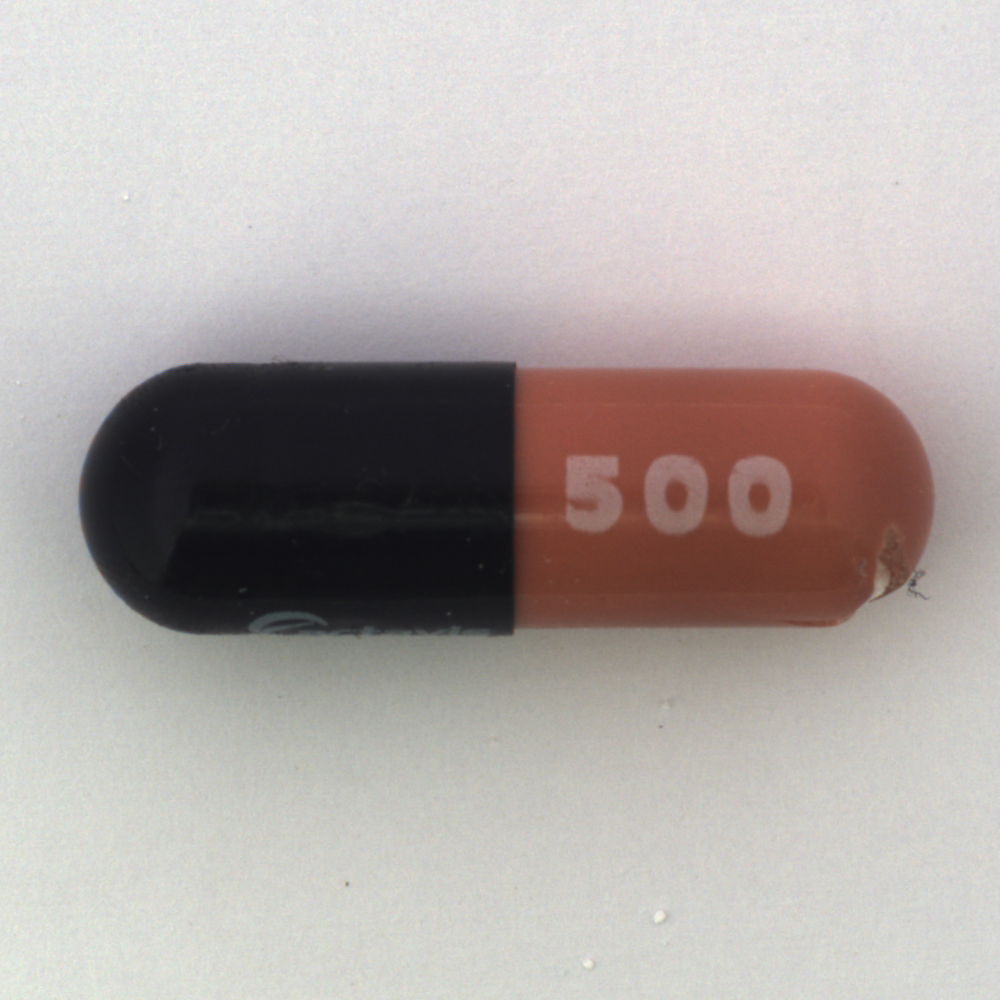
\includegraphics[width=.85cm]{figures/capsule-original.png}};
\node[tinylabel,text=raBlue] at (10.4,3.18) {returned};
% Missing.
\draw[draw=black!50,line width=2.2pt] (5.1,2.06) -- (5.1,2.84);
\node[anchor=west,font=\small\bfseries,text=black!65] at (5.25,2.59) {Missing};
\node[anchor=west,font=\footnotesize] at (5.25,2.21) {Original not in pool};
\node[photo] at (8.3,2.45) {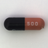
\includegraphics[width=.85cm]{figures/capsule-preview.png}};
\draw[arr] (8.88,2.45) -- (9.67,2.45);
\draw[draw=black!40,dashed,line width=.65pt] (9.975,2.135) rectangle (10.825,2.985);
\draw[draw=black!45,line width=.6pt] (10.13,2.29) -- (10.67,2.83) (10.13,2.83) -- (10.67,2.29);
\node[tinylabel] at (10.4,1.98) {not returned};
% Unavailable: an existing image is blocked from release.
\draw[draw=raOrange,line width=2.2pt] (5.1,.86) -- (5.1,1.64);
\node[anchor=west,font=\small\bfseries,text=raOrange] at (5.25,1.39) {Unavailable};
\node[anchor=west,font=\footnotesize] at (5.25,1.01) {Original not released};
\node[photo] at (8.3,1.25) {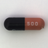
\includegraphics[width=.85cm]{figures/capsule-preview.png}};
\draw[arr,draw=raOrange] (8.88,1.25) -- (9.67,1.25);
\node[photo,opacity=.48] at (10.4,1.36) {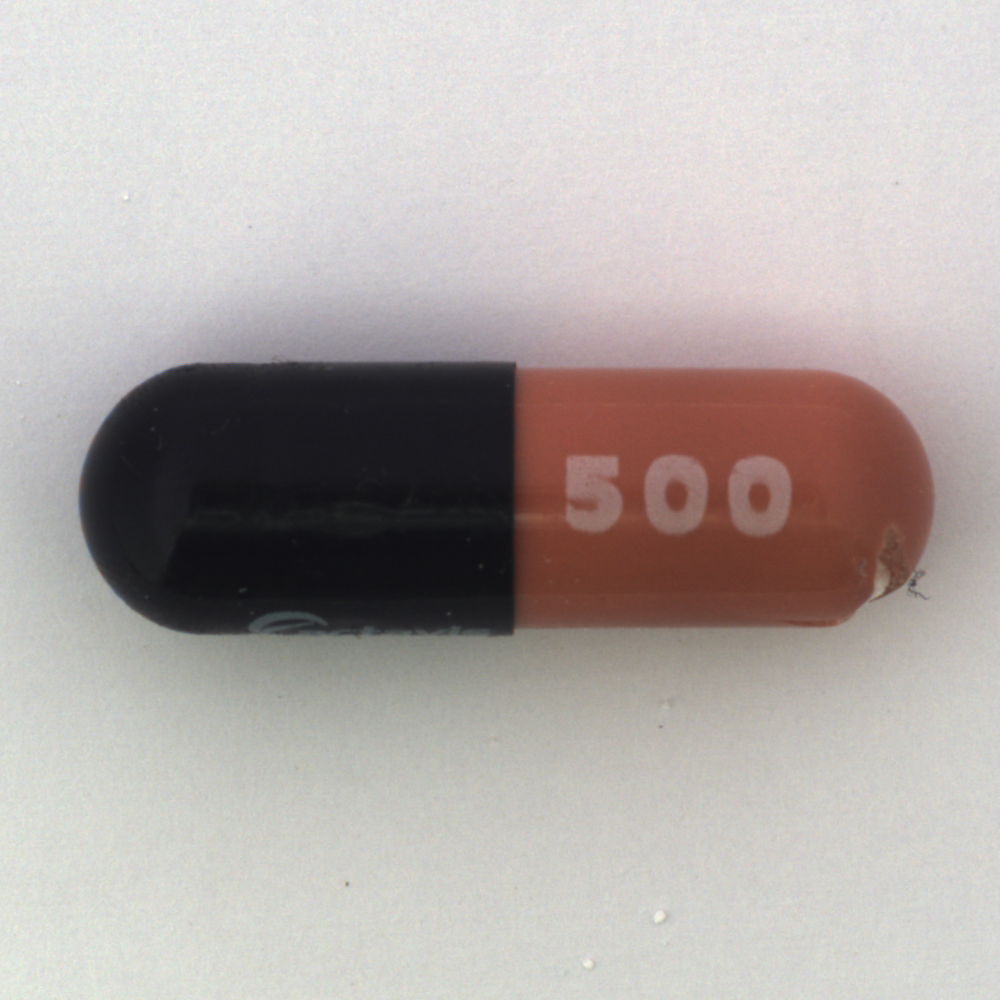
\includegraphics[width=.85cm]{figures/capsule-original.png}};
\draw[draw=raOrange,line width=1pt] (10.0,.96) -- (10.8,1.76);
\node[tinylabel,text=raOrange] at (10.4,.78) {not returned};
\node[font=\scriptsize,text=black!65] at (8.2,.27) {Last three settings share the same preview and request.};
% (c) Concrete image operations rather than backend components.
\node[anchor=west,font=\footnotesize] at (12.03,6.02) {Choose the observation needed for the claim.};
\node[font=\footnotesize\bfseries] at (13.1,5.55) {Crop / inspect};
\node[font=\footnotesize\bfseries] at (15.95,5.55) {Compare / ground};
% Crop x=[780,960], y=[470,670], source origin top-left.
\node[photo] at (13.1,4.73) {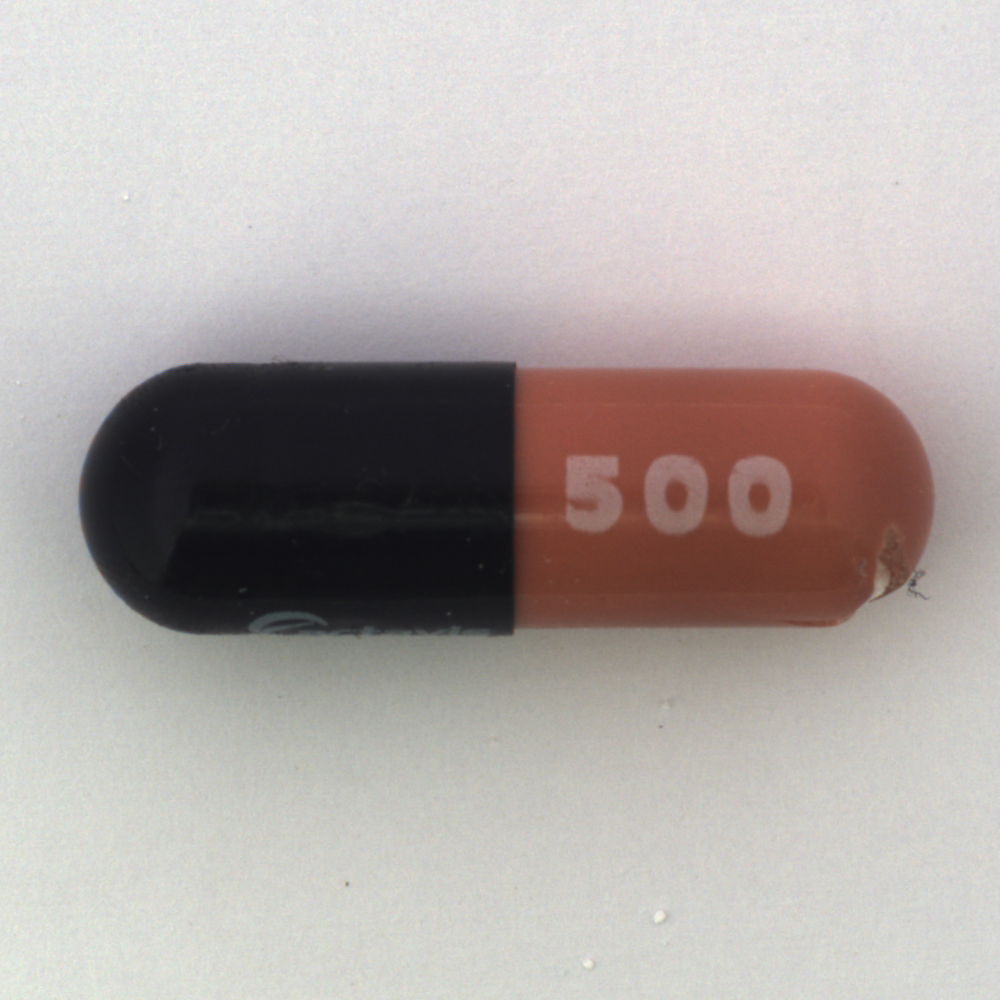
\includegraphics[height=1.3cm,trim=780bp 330bp 40bp 470bp,clip]{figures/capsule-original.png}};
\node[photo] at (15.27,4.73) {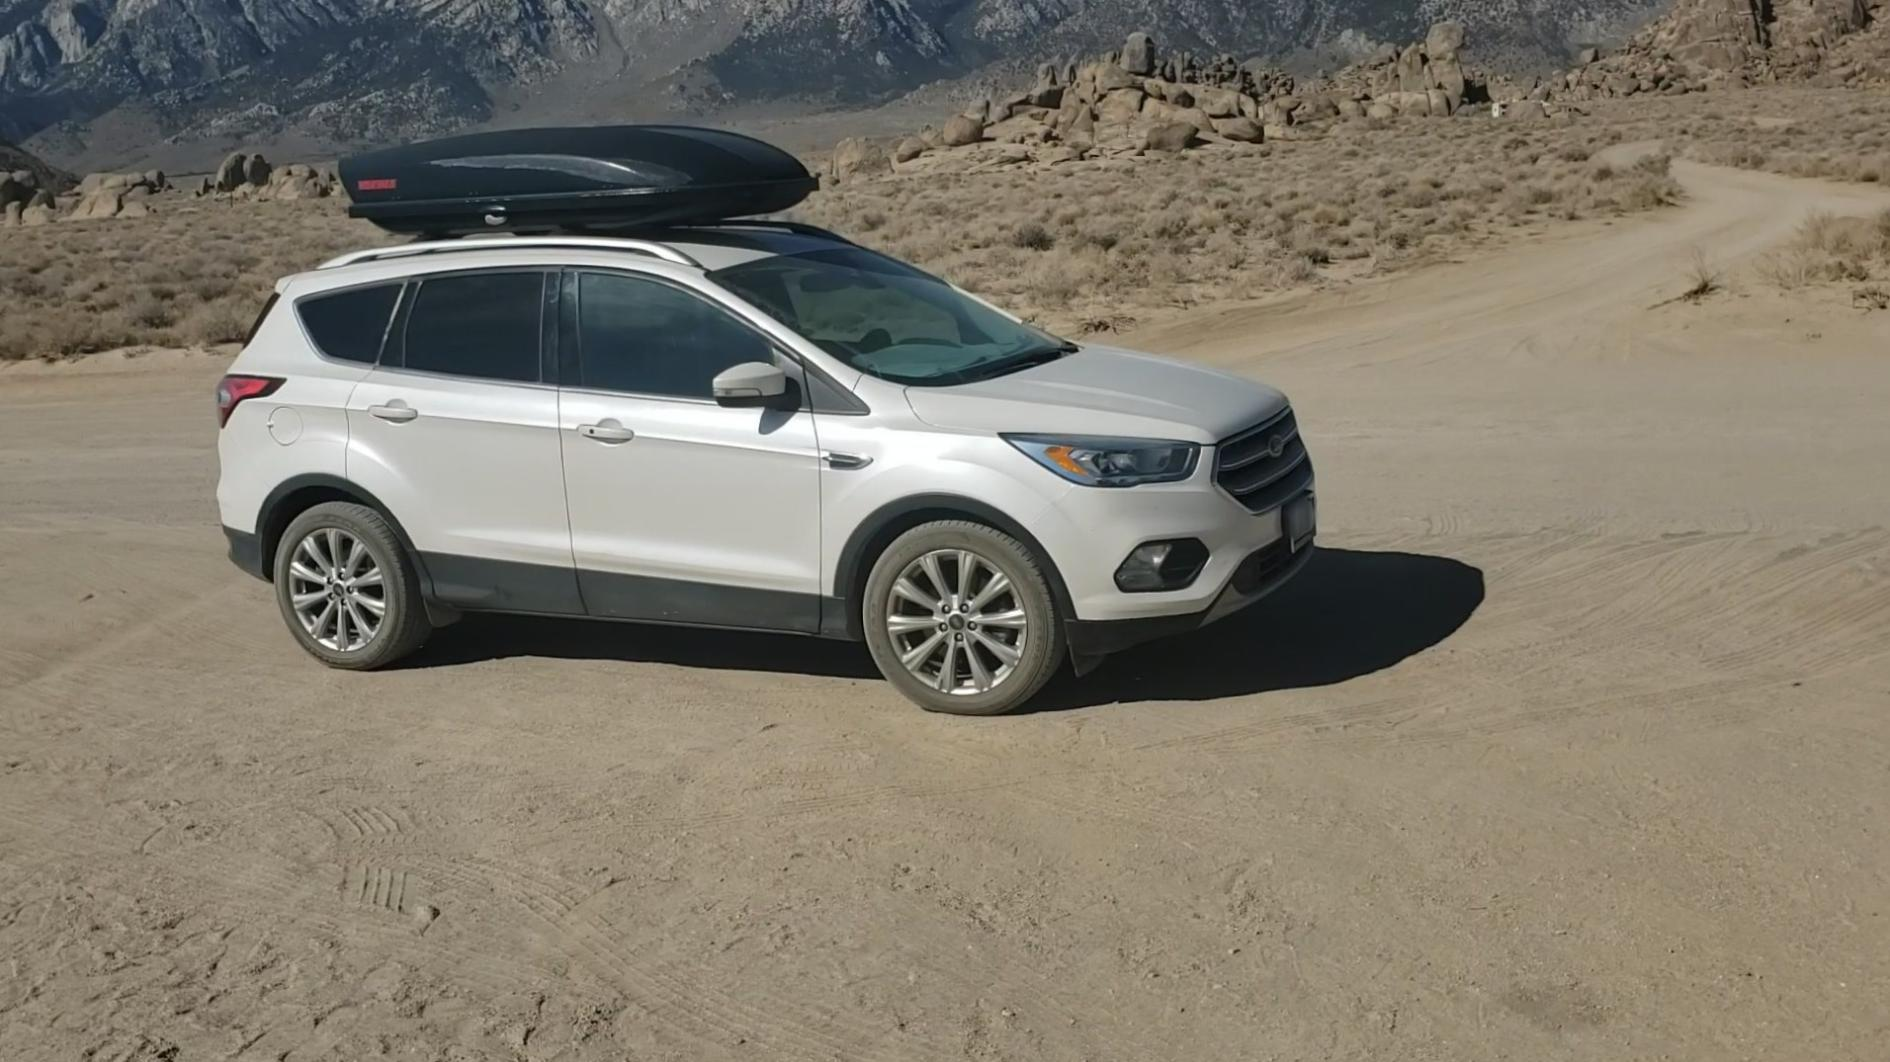
\includegraphics[width=1.18cm]{figures/case-vehicle-a.jpg}};
\node[photo] at (16.65,4.73) {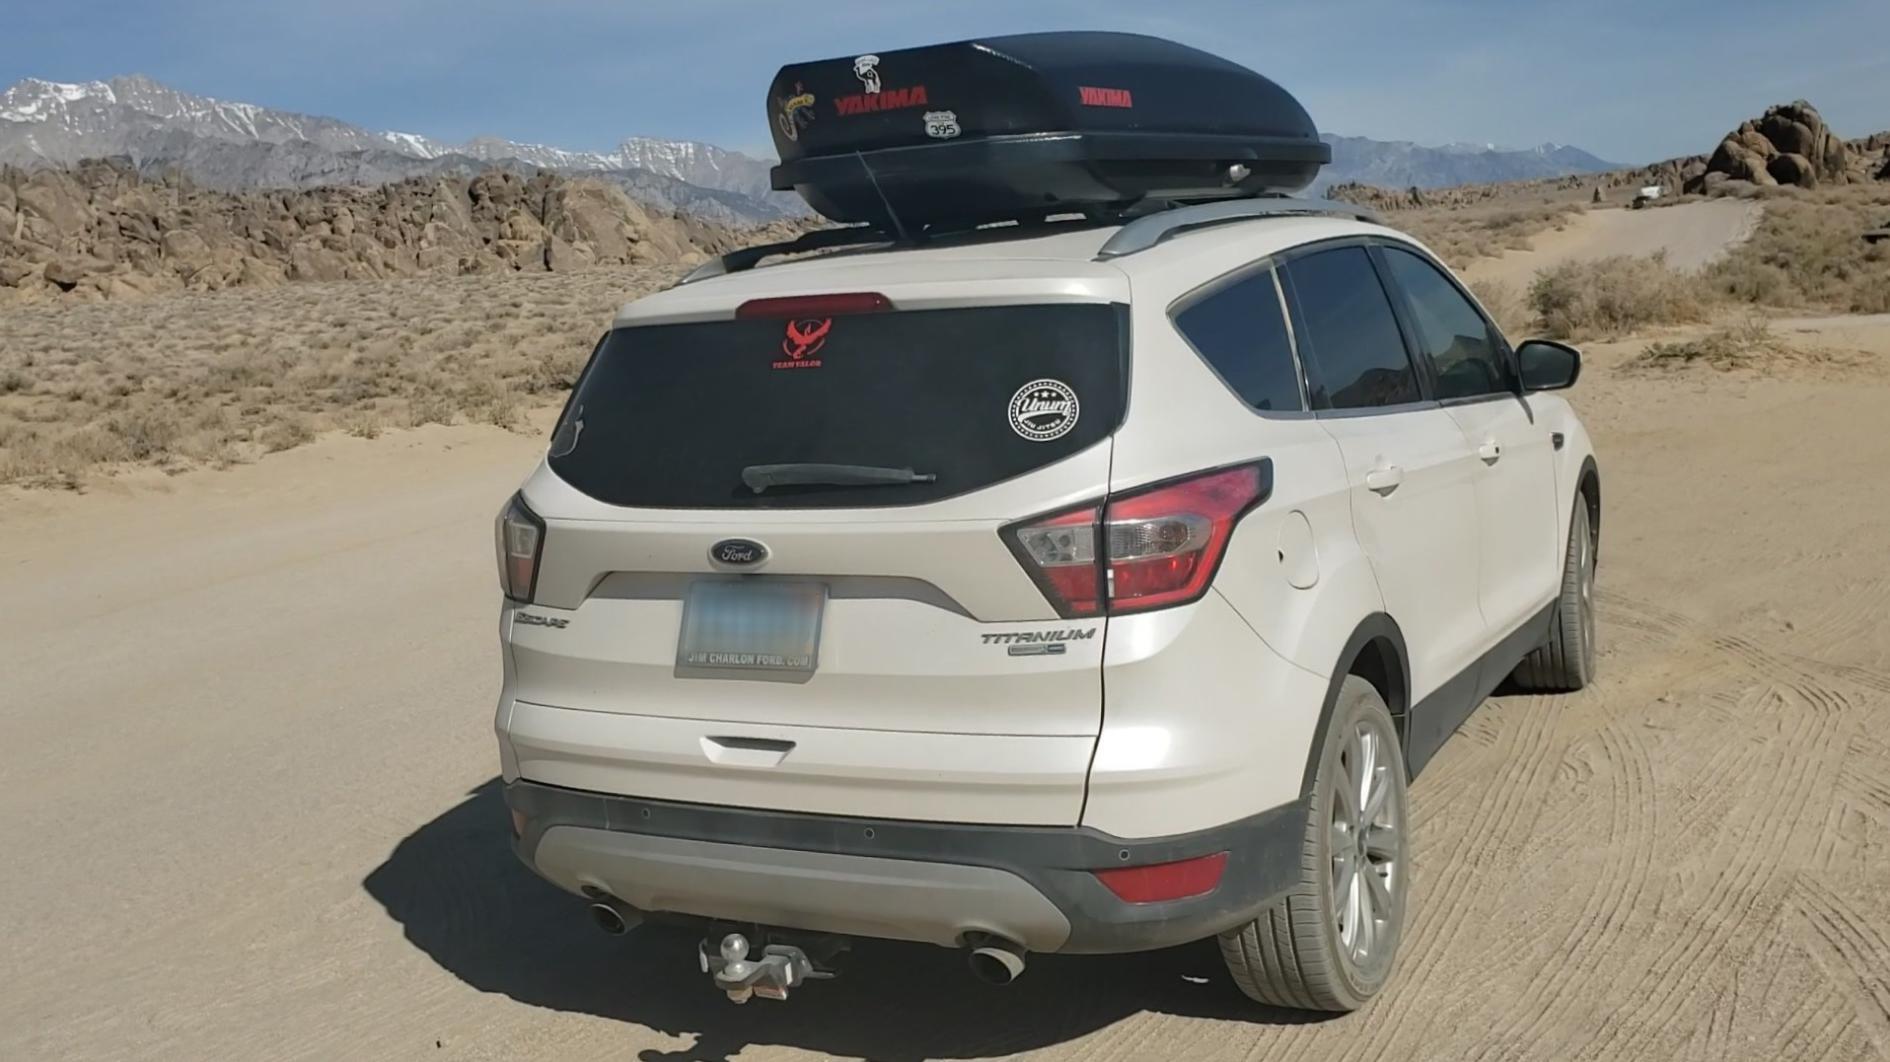
\includegraphics[width=1.18cm]{figures/case-vehicle-b.jpg}};
\draw[<->,draw=raBlue,line width=.6pt] (15.9,4.73) -- (16.0,4.73);
\node[note] at (13.1,3.94) {Existing pixels};
\node[note] at (15.95,3.94) {Across-image check};
\node[font=\footnotesize\bfseries,text=raBlue] at (13.1,3.35) {Request original};
\node[font=\footnotesize\bfseries,text=raBlue] at (15.95,3.35) {Request view};
\node[photo] at (13.1,2.38) {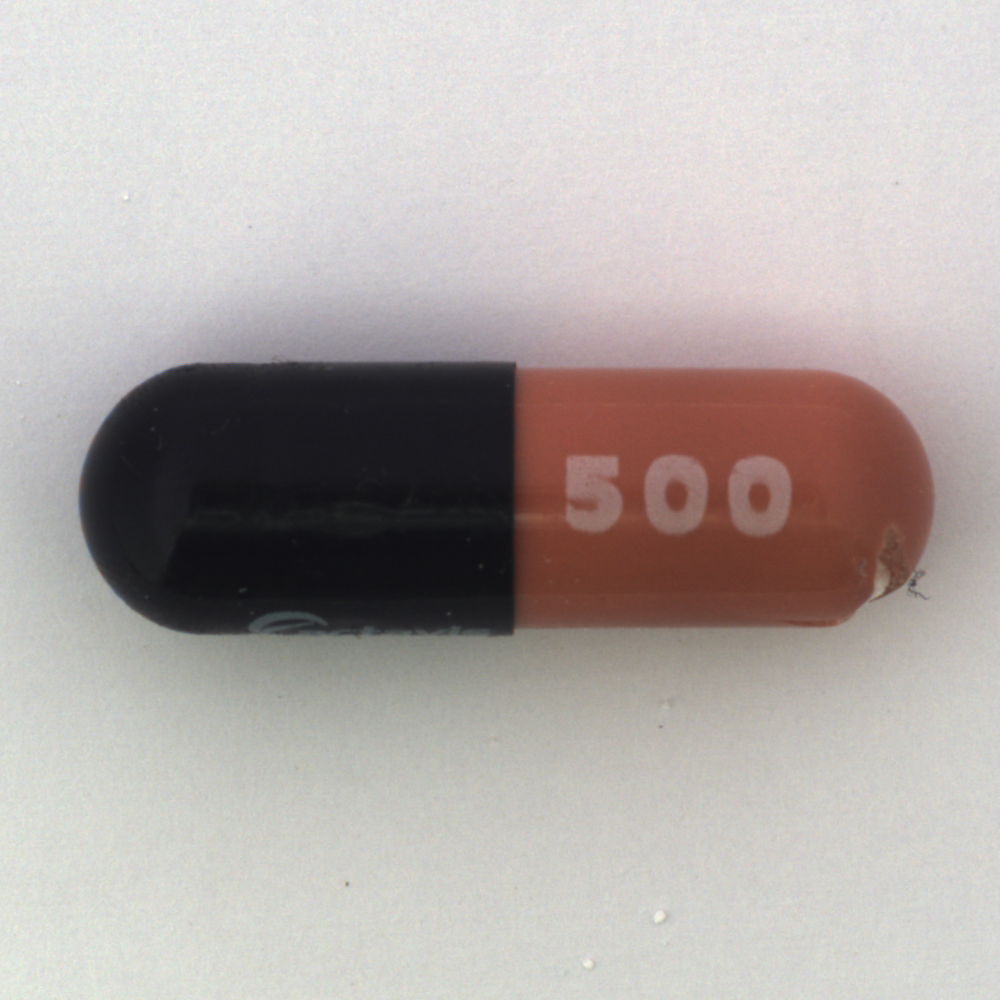
\includegraphics[width=1.45cm]{figures/capsule-original.png}};
\node[photo] at (15.95,2.38) {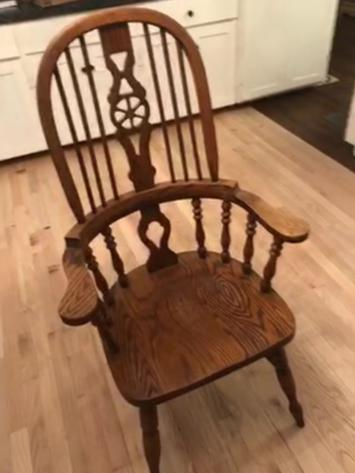
\includegraphics[height=1.5cm]{figures/chair-a-new.jpg}};
\node[note] at (13.1,1.4) {Recorded image};
\node[note] at (15.95,1.4) {Recorded angle};
\draw[rule] (12.03,1.05) -- (17.37,1.05);
\node[anchor=west,font=\footnotesize] at (12.03,.73)
  {\textbf{Finish:} answer + image/region references};
\node[anchor=west,font=\footnotesize,text=raOrange] at (12.03,.25)
  {Supported / Refuted / Need more evidence};
\end{tikzpicture}%
\endgroup%
